\documentclass[12pt]{article}

\usepackage[margin=3cm]{geometry}
\usepackage{graphicx}
\usepackage{pdfpages}
\usepackage{minted}

\author{Pablo Vargas Bermúdez}

\begin{document}
\pagestyle{empty}
\includepdf[pages=-]{Portada}

\section*{Planteamiento}
Una vez realizado el tutorial de la base de datos agrega algunos
registros a tu nueva base.  Sigue la Guia el ejercicio anterior para
crear un programa que se conecte a tu base de datos.

Envía un archivo PDF que contenga una hoja de presentación, la
descripción de la tarea, el código fuente de la solución y las
capturas de pantalla de las bases de datos que realizaste, mostrando
la información almacenada en las tablas que son consultadas, anexa
también las pantallas necesarias donde muestres el correcto
funcionamiento del programa funcionamiento.

\textbf{NOTA:} No es conectarse a cualquier base de datos, es a la que viene en
el tutorial y la descrita en el PDF de la liga anterior. Puedes usar
cualquier manejador de BD que tengas disponible, no necesariamente
Derby.

\section*{Código}

\subsection*{Conexión}
\inputminted{Java}{DataBase.java}
\subsection*{Gui}
\inputminted{Java}{Gui.java}
\subsection*{Prueba}
\inputminted{Java}{PruebaDataBase.java}

\section*{Ejecución}
\begin{figure}[ht]
  \centering
  \includegraphics[width=\textwidth]{figures/tabla.png}
  \caption{Tabla COLLEAGUES}
\end{figure}

\begin{figure}[ht]
  \centering
  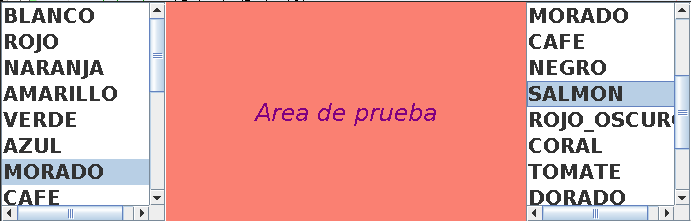
\includegraphics[width=\textwidth]{figures/run1.png}
  \caption{Primera prueba}
\end{figure}

\begin{figure}[ht]
  \centering
  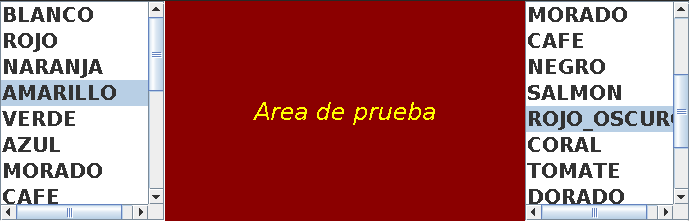
\includegraphics[width=.5\textwidth]{figures/run2.png}
  \caption{Segunda prueba}
\end{figure}

\begin{figure}[ht]
  \centering
  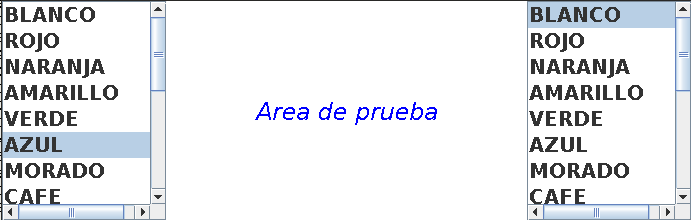
\includegraphics[width=.5\textwidth]{figures/run3.png}
  \caption{Tercera prueba}
\end{figure}

\begin{figure}[ht]
  \centering
  \includegraphics[width=\textwidth]{figures/run4-1.png}
  \caption{Cuarta prueba, primer prompt}
\end{figure}

\begin{figure}[ht]
  \centering
  \includegraphics[width=\textwidth]{figures/run4-2.png}
  \caption{Cuarta prueba, sedundo prompt}
\end{figure}

\end{document}
